\documentclass[12pt, a4paper, oneside]{ctexart}
\usepackage{amsmath, amsthm, amssymb, bm, color, framed, graphicx, hyperref, mathrsfs, geometry}
\usepackage{algorithm, algorithmicx, algpseudocode}

\title{\textbf{机器学习第一次作业}}
\author{汪隽立\ 2021012957}
\date{\today}
\linespread{1.5}
\definecolor{shadecolor}{RGB}{241, 241, 255}
\newcounter{problemname}
\newenvironment{problem}[1]{\begin{shaded}\par\noindent\textbf{题目 #1. }}{\end{shaded}\par}
\newenvironment{solution}[1]{\par\noindent\textbf{解答 #1. }\par}{\par}
\newenvironment{note}{\par\noindent\textbf{题目\arabic{problemname}的注记. }}{\par}

\geometry{a4paper,scale=0.8}
\begin{document}

\maketitle

\par\noindent \textbf{注:}报告中只对作业要求的题目作出解答。代码填空部分除非特殊情况,不在报告中赘述。

\begin{solution}{2.2.1}
    \begin{equation}
        J(\theta) = \frac{1}{m} \| y - X\theta \| ^ 2 + \lambda \theta ^ \top \theta \nonumber
    \end{equation}
    其中$X \in \mathbb{R}^{m\times (d+1)}$,$y \in \mathbb{R}^{m}$,$\theta \in \mathbb{R}^{d+1}$。
\end{solution}

\begin{solution}{2.2.3}
    \begin{equation}
        \frac{\partial{J(\theta)}}{\partial \theta} = \frac{2}{m} X^\top (X\theta - y) + 2\lambda \theta \nonumber
    \end{equation}
    其中用到了有关矩阵求导的公式:
    \begin{align}
        &\frac{\partial{\mathbf{X}\theta}}{\partial{\theta}} = \mathbf{X}^\top \nonumber \\
        &\frac{\partial{\| x \|^2}}{\partial{x}} = 2x \nonumber
    \end{align}
\end{solution}

\begin{solution}{2.2.6}
    在我们的处理中,偏置项$b = \theta_{d+1}$($\theta_{d+1}$表示$\theta$ 的第$i+1$个分量)。而
    \begin{equation}
        \frac{\partial{J(\theta)}}{\partial \theta_{d+1}} = \frac{2}{m} X^\top \left(X\theta - y\right)_{d+1} + 2\lambda \theta_{d+1} \nonumber
    \end{equation}
    如果将$x$添加的额外维度置为$B$,那么$X^\top$的第$d+1$行为$\left( B, B, \dots, B \right)$,$X\theta - y = \left( A_1 + B\theta_{d+1}, A_2 + B\theta_{d+1}, \dots, A_m + B\theta_{d+1}\right)^\top$,其中$A_i = \sum_{k=1}^{d} x_{ik}\theta_k$。故在偏导数的计算中,均方误差带来的梯度为
    \begin{equation}
        \frac{2}{m} X^\top (X\theta - y)_{d+1} = \sum_{i=1}^{m} B \times A_i + mB^2\theta_{d+1} \nonumber
    \end{equation}
    可以看出这一项的量级至少是$O(B)$的。而正则化带来的梯度为$2\lambda \theta_{d+1}$,一方面$\| \theta_{d+1} \|$非常小,另一方面$B$非常大。我们有:
    \begin{equation}
        \| 2\lambda \theta_{d+1} \| \ll \| \frac{2}{m} X^\top (X\theta - y)_{d+1} \| \nonumber
    \end{equation}
    也就是说,此时正则化对偏置项梯度的影响可以忽略不计。
\end{solution}

\begin{solution}{2.3.1}
    \begin{equation}
        J(\theta + \eta h) - J(\theta) \approx \eta \left< \nabla J(\theta), h \right> \nonumber
    \end{equation}
    其中内积为$\mathbb{R}^n$上的内积。可以看出当梯度与$h$反向时,函数减少得最多,所以$h$的前进方向应当为梯度的反方向。
\end{solution}

\begin{solution}{2.3.2}
    \begin{equation}
        \theta^\prime = \theta - \eta \nabla J(\theta) \nonumber
    \end{equation}
\end{solution}

\begin{solution}{2.3.4}
    能使实验结果收敛的学习率如下,分别为$0.001, 0.005, 0.01, 0.05$":
    \begin{figure}[htbp]
        \centering
        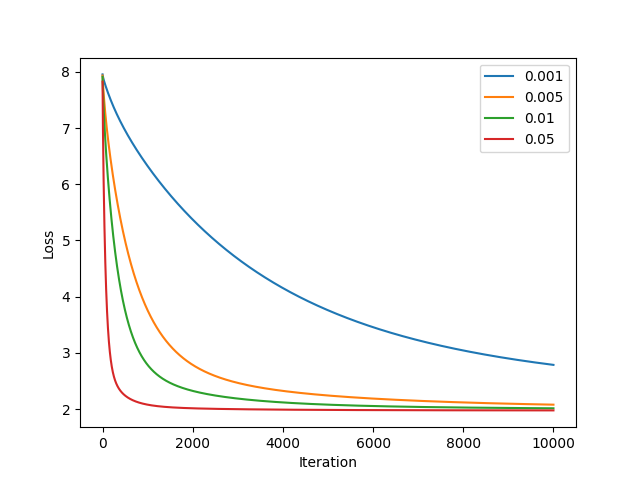
\includegraphics[width=.9\textwidth]{pic/Figure_2.png}
    \end{figure}
    而当学习率为$0.1, 0.5$时,这时$\lambda \gg O(\frac{1}{L})$,$L$为目标函数的Lipschitz常数,梯度下降算法不再收敛。
    \begin{figure}[htbp]
        \begin{minipage}[t]{0.5\linewidth}
        \centering
        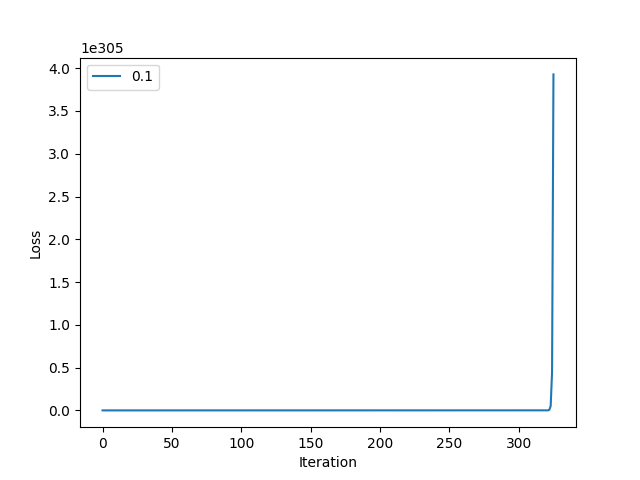
\includegraphics[width=1.0\textwidth]{pic/Figure_3.png}
        \end{minipage}%
        \begin{minipage}[t]{0.5\linewidth}
        \centering
        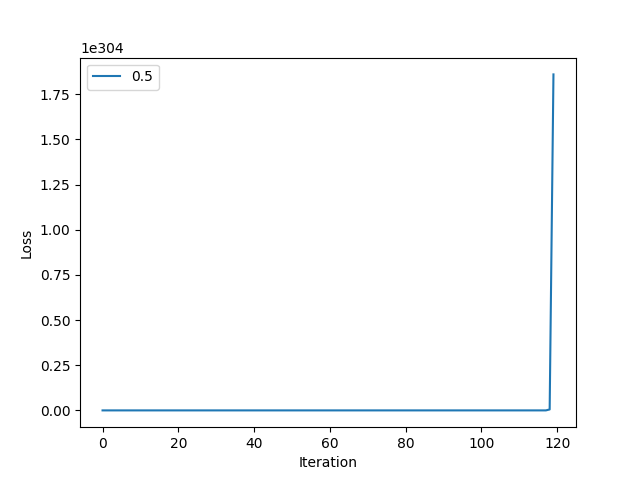
\includegraphics[width=1.0\textwidth]{pic/Figure_4.png}
        \end{minipage}
    \end{figure}
        
\end{solution}

\begin{solution}{2.4.1}
    \begin{equation}
        \nabla J_{SGD}(\theta) = \frac{2}{n} \sum_{k=1}^{n} x_{i_k}^\top(\theta^\top x_{i_k} - y_{i_k}) + 2\lambda \theta \nonumber
    \end{equation}
\end{solution}

\begin{solution}{2.4.2}
    \begin{align}
        \mathbb{E}_{i_1, \dots, i_n} \left[ \nabla J_{SGD} (\theta) \right] & = \mathbb{E} \left[ \frac{2}{n} \sum_{k=1}^{n}  x_{i_k}^\top(\theta^\top x_{i_k} - y_{i_k}) \right]  + 2\lambda \theta \nonumber \\ 
        \text{(期望的线性性)} & = \frac{2}{n} \sum_{k=1}^{n} \mathbb{E}_{x_{i_k} \sim D} \left[  x_{i_k}^\top(\theta^\top x_{i_k} - y_{i_k}) \right] + 2\lambda \theta \nonumber \\
        \text{(i.i.d.)}& = 2\mathbb{E}_{x \sim D}\left[ x^\top (\theta^\top x - y) \right] + 2\lambda \theta \nonumber \\
        & = \frac{2}{m} \sum_{x_i \in \mathcal{X}} \left[ x_i^\top (\theta^\top x_i - y_i) \right] + 2\lambda \theta \nonumber \\
        & = \nabla J(\theta) \nonumber
    \end{align}
\end{solution}

\begin{solution}{2.4.4}
    选取学习率为$0.01$,$batchsize = \{1, 10, 20, 50, 100\}$进行实验:
    \begin{figure}[htbp]
        \centering
        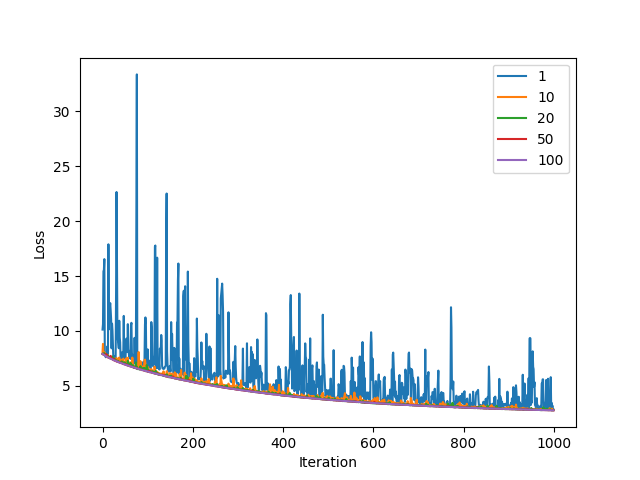
\includegraphics[width=.7\textwidth]{pic/Figure_5.png}
        \caption{不同batchsize对SGD的影响}
    \end{figure}
    可以看到,随着$batchsize$的增大,训练误差有更好的稳定性。不过训练效率也有所下降,$batchsize = 100$即全批量训练。
\end{solution}

\begin{solution}{2.4.5}
    选取学习率为$0.01$,$batchsize = 20$,$\lambda = \{ 10^{-7}, 10^{-5}, 10^{-3}, 10^{-1}, 1, 10, 100\}$进行SGD实验:
    \begin{figure}[htbp]
        \centering
        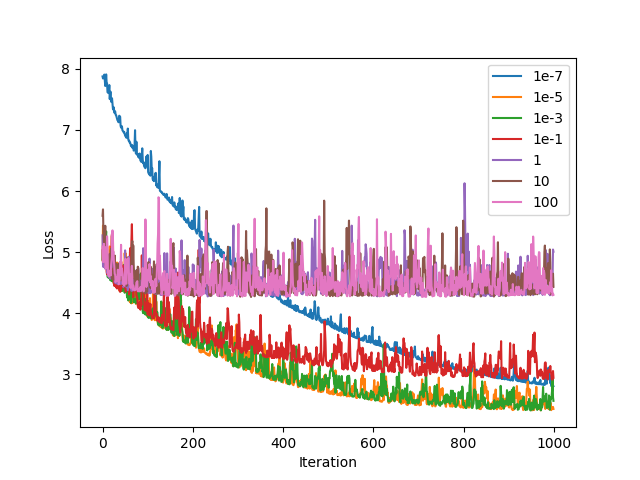
\includegraphics[width=.7\textwidth]{pic/Figure_6.png}
        \caption{不同$\lambda$对SGD的影响}
    \end{figure}
    可以看出,当$\lambda$过大时,\textbf{模型基本没有学习能力}。而适当的$\lambda = \{10^{-5}, 10^{-3}\}$能够提高模型的泛化能力。
\end{solution}

\begin{solution}{2.6.1}
    \begin{equation}
        H = \frac{2}{m} X^\top X + 2\lambda I \nonumber
    \end{equation}
    其中$X^\top X$半正定,再加上一个正定阵,自然是正定阵,故奇异。
\end{solution}

\begin{solution}{2.6.2}
    \begin{figure}[htbp]
        \centering
        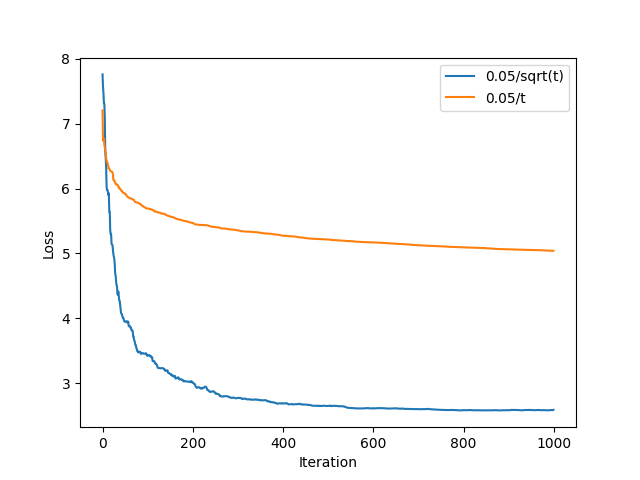
\includegraphics[width=.7\textwidth]{pic/Figure_7.png}
    \end{figure}
    从结果上看,牛顿迭代法大大减少了收敛所需要的迭代步数。不论是GD还是SGD,其需要的步数都大约为1000步,而牛顿迭代法基本上只需要100步就可收敛。\\
    然而,牛顿迭代法也牺牲了一定的计算复杂度。在每一步迭代中,牛顿迭代法牺牲了更多的时间计算Hessian矩阵的逆矩阵。而GD和SGD只需要计算梯度,计算复杂度较低。实验表明,在迭代次数为10000时,牛顿迭代法所需要的时间为1.48秒,而SGD需要0.22秒($batchsize=20$)。总的来说牛顿迭代法在时间上能使收敛速度变快,但其单步的速度实际上是不如SGD的。
\end{solution}

\begin{solution}{3.1.1}
    \begin{equation}
        \partial J(w) = 
        \begin{cases}
            -yx & \text{if $yw^\top x < 1$} \\
            0 & \text{if $yw^\top x > 1$} \\ 
            \text{any number between $0$ and $-yx$} & \text{if $yw^\top x = 1$}
        \end{cases} \nonumber
    \end{equation}
\end{solution}

\begin{solution}{3.1.2}
    假设$f$不凸,i.e.存在$x_0, y_0 \in dom(f)$,$\lambda \in [0, 1]$,使得
    \begin{equation}
        \lambda f(x_0) + (1 - \lambda) f(y_0) < f(\lambda x_0 + (1 - \lambda) y_0) \nonumber
    \end{equation}
    因为$f$的次梯度处处存在,所以在$\lambda x_0 + (1 - \lambda) y_0$处有
    \begin{align}
        & f(x_0) \geq f(\lambda x_0 + (1 - \lambda) y_0) - (1 - \lambda) g^\top(y_0 - x_0) \\
        & f(y_0) \geq f(\lambda x_0 + (1 - \lambda) y_0) + \lambda g^\top(y_0 - x_0)
    \end{align}
    $\lambda \times (1) + (1 - \lambda) \times (2)$,得
    \begin{equation}
        \lambda f(x_0) + (1 - \lambda) f(y_0) \geq f(\lambda x_0 + (1 - \lambda) y_0) \nonumber
    \end{equation}
    这与$f$不凸的假设矛盾。故$f$为凸函数。
\end{solution}

\begin{solution}{3.2.1}
    选择合适的次梯度为
    \begin{equation}
        g = 
        \begin{cases}
            -y_ix_i & \text{if $y_iw^\top x_i < 0$} \\
            0 & \text{Others}
        \end{cases}
        \nonumber
    \end{equation}
    这样,当SSGD算法随机采样到$(x_i, y_i)$时,$w$的更新如下:
    \begin{equation}
        w^{(k+1)} =
        \begin{cases}
            w^{(k)} & \text{if $y_iw^\top x_i > 0$(分类正确)} \\
            w^{(k)} + y_ix_i & \text{if $y_iw^\top x_i < 0$(分类错误)}
        \end{cases}
        \nonumber
    \end{equation}
    这和感知机算法的更新是一致的。假设SSGD迭代的轮次足够大,可以认为$w$和感知机算法得到的结果一样,都能正确地线性区分数据。
\end{solution}

\begin{solution}{3.2.2}
    由于$w$的初始值为$(0, \dots, 0)$,而每一步更新$w$用到的公式为
    \begin{equation}
        w^{(k+1)} =
        \begin{cases}
            w^{(k)} & \text{if $y_iw^\top x_i > 0$(分类正确)} \\
            w^{(k)} + y_ix_i & \text{if $y_iw^\top x_i < 0$(分类错误)}
        \end{cases}
        \nonumber
    \end{equation}
    其中$y_i \in \{-1, +1\}$。故$w$自然是$\{x_i\}_{i=1}^n$的线性组合,$\alpha_i$即为更新过程中加上$y_ix_i$的次数(或者可以用数学归纳法/表示定理说明这件事)。
\end{solution}

\begin{solution}{3.3.1}
    \begin{align}
        L(w, b, \xi, \alpha, \mu) = & \  \frac{\lambda}{2} \| w \|^2 + \frac{1}{m} \sum_{i=1}^{m} \xi_i + \sum_{i=1}^{m} \alpha_i (1 - y_i(w^\top x_i + b) - \xi_i) - \sum_{i=1}^{m} \mu_i \xi_i \nonumber \\
        & \text{where}\quad  \alpha_i > 0, \mu_i > 0, i = 1, 2, \dots, n \nonumber
    \end{align}
\end{solution}

\begin{solution}{3.3.2}
    在3.3.1的拉格朗日方程中,令
    \begin{align}
        & \frac{\partial L}{\partial w} = \lambda w - \sum_{i=1}^{m} \alpha_i y_i x_i = 0 \nonumber \\
        & \frac{\partial L}{\partial b} = -\sum_{i=1}^{m} \alpha_i y_i = 0 \nonumber \\ 
        & \frac{\partial L}{\partial \xi_i} = \frac{1}{m} - \alpha_i - \mu_i = 0 \nonumber
    \end{align}
    得
    \begin{align}
        & w = \frac{1}{\lambda} \sum_{i=1}^{m} \alpha_i y_i x_i \nonumber \\
        & \sum_{i=1}^{m} \alpha_i y_i = 0 \nonumber \\
        & \alpha_i = \frac{1}{m} - \mu_i \nonumber
    \end{align}
    带入拉格朗日方程,得
    \begin{equation}
        \Pi(\alpha, \mu) = \sum_{i=1}^{m} \alpha_i - \frac{1}{2\lambda}\sum_{i,j=1}^{m}\alpha_i \alpha_j y_i y_j \left< x_i, x_j\right> \nonumber
    \end{equation}
    Dual Problem即为
    \begin{align}
        & \max_{\alpha} \Pi(\alpha, \mu) \nonumber \\
        s.t. \quad & 0 \leq \alpha_i \leq \frac{1}{m} \nonumber \\
        \quad \quad & \sum_{i=1}^{m} \alpha_i y_i = 0, \quad i = 1, 2, \dots, m \nonumber
    \end{align}
\end{solution}

\begin{solution}{3.3.3}
    Primal Problem: 
    \begin{align}
        \min_{w, b, \xi} \ & \frac{\lambda}{2} \| w \|^2 + \frac{1}{m} \sum_{i=1}^{m} \xi_i \nonumber \\
        s.t. \quad & y_i(w^\top \Phi(x_i) + b) \geq 1 - \xi_i \nonumber \\
        & \xi_i \geq 0, \quad i = 1, 2, \dots, m \nonumber
    \end{align}
    Dual Problem:
    \begin{align}
        \max_{\alpha} \ & \sum_{i=1}^{m} \alpha_i - \frac{1}{2\lambda} \sum_{i,j=1}^{m}\alpha_i \alpha_j y_i y_j k(x_i, x_j)\nonumber \\
        s.t. \quad & 0 \leq \alpha_i \leq \frac{1}{m} \nonumber \\
        \quad \quad & \sum_{i=1}^{m} \alpha_i y_i = 0, \quad i = 1, 2, \dots, m \nonumber
    \end{align}
\end{solution}

\begin{solution}{3.3.4}
    记$f(w) = \frac{\lambda}{2} \| w \| ^ 2$。由于$f$关于$w$是凸函数,故$f$的梯度即为其次梯度。又由前我们已经计算出Hinge Loss的次梯度为:
    \begin{equation}
        \partial (\max \{ 0, 1 - y_i(w^\top x_i + b) \})_w = 
        \begin{cases}
            -y_ix_i & \text{if $y_iw^\top x_i < 1$} \\
            0 & \text{if $y_iw^\top x_i > 1$}
        \end{cases} \nonumber
    \end{equation}
    \begin{equation}
        \partial (\max \{ 0, 1 - y_i(w^\top x_i + b) \})_b = 
        \begin{cases}
            -y_i & \text{if $y_iw^\top x_i < 1$} \\
            0 & \text{if $y_iw^\top x_i > 1$}
        \end{cases} \nonumber
    \end{equation}
    而次梯度的和仍然是次梯度,$\partial J_{i|w} = \lambda w + \partial (\max \{ 0, 1 - y_i(w^\top x_i + b) \})_w$,$\partial J_{i|b} = \partial (\max \{ 0, 1 - y_i(w^\top x_i + b) \})_b$。此即要证明的等式。
\end{solution}

\begin{solution}{3.3.5}
    见Algorithm 1。
    \begin{algorithm}[htbp]
        \caption{SSGD for SVM}
        \begin{algorithmic}[width=0.8\textwidth]
            \State 输入:训练集$(x_1, y_1), \dots, (x_n, y_n) \in \mathbb{R}^d \times \{-1, 1\}$
            \State Initialize $w$, $b$, $BS=\text{Batch Size}$, $\eta = \text{Learning Rate}$, $T = \text{Iterations}$
            \For {$t = 1, 2, \dots, T$}
                \State Randomly sample a minibatch $\{(x_i, y_i)\}_{i=1}^{BS}$
                \State Calculate subgradient on minibatch:
                \State $\partial J_w = \frac{1}{BS} \sum_{i=1}^{BS} \partial J_{i|w}$, $\partial J_b = \frac{1}{BS} \sum_{i=1}^{BS} \partial J_{i|b}$
                \State $w = w - \eta \partial J_w$, $b = b - \eta \partial J_b$
            \EndFor
            \State 输出:$w$, $b$
        \end{algorithmic}
    \end{algorithm}
\end{solution}

\begin{solution}{3.3.6}
    只需证明最优解中,必有$\xi_i \geq 0$。假设最优解的某个$\xi_i < 0$。现在令$\xi_i^\prime = 0$,有$y_i(w^\top x_i + b) \geq 1 - \xi_i \geq 1 - \xi_i^\prime$。也就是说将$\xi_i$替换成$\xi_i^\prime = 0$,仍然能满足约束条件,但目标函数的值减少了。这与最优解的假设矛盾。
\end{solution}

\begin{solution}{3.3.7}
    Lagrange Function: 
    \begin{align}
        L(w, b, \xi, \alpha) = & \ \frac{\lambda}{2} \| w \|^2 + \frac{1}{m} \sum_{i=1}^{m} \xi_i^2 + \sum_{i=1}^{m} \alpha_i (1 - y_i(w^\top x_i + b) - \xi_i) \nonumber \\
        & \text{where}\quad  \alpha_i > 0, i = 1, 2, \dots, n \nonumber
    \end{align} \par
    Dual Problem:
    \begin{equation}
        \Pi(\alpha) = \sum_{i=1}^{m} (\alpha_i - \frac{m}{4}\alpha_i ^ 2) - \frac{1}{2\lambda}\sum_{i,j=1}^{m}\alpha_i \alpha_j y_i y_j \left< x_i, x_j\right> \nonumber
    \end{equation}
\end{solution}

\begin{solution}{3.4.2}
    首先列出训练损失随着迭代次数的变化:
    \begin{figure}
        \centering
        \caption{SGD训练损失随迭代次数的变化}
        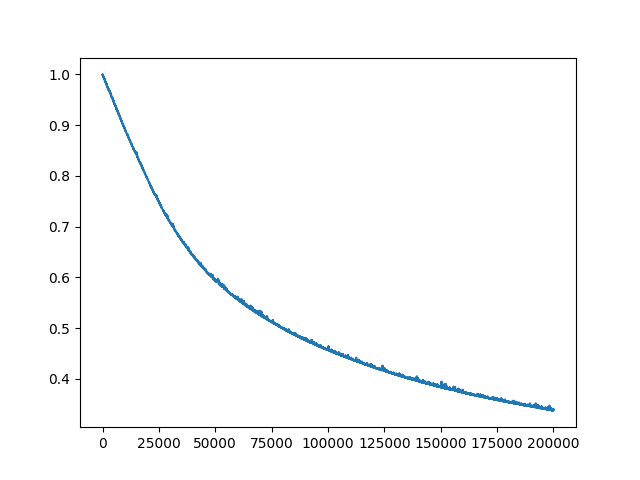
\includegraphics[width=.7\textwidth]{pic/Figure_8.png}
    \end{figure}
    以下列出不同学习率对验证集准确率的影响:
    \begin{table}[h!]
        \begin{center}
          \caption{不同学习率对验证集准确率}
          \begin{tabular}{l|c} % <-- Alignments: 1st column left, 2nd middle and 3rd right, with vertical lines in between
            \textbf{学习率} & \textbf{验证集上准确率} \\
            \hline
            0.001 & 0.66\\
            0.005 & 0.83\\
            0.01 & 0.85\\
            0.05 & 0.85\\
            0.1 & 0.86\\
            0.5 & 0.83\\
          \end{tabular}
        \end{center}
    \end{table}
    于是选择学习率为$0.1$。接下来列出不同$\lambda$对验证集准确率的影响:
    \begin{table}[h!]
    \begin{center}
        \caption{不同$\lambda$对验证集准确率}
          \begin{tabular}{l|c} % <-- Alignments: 1st column left, 2nd middle and 3rd right, with vertical lines in between
            \textbf{$\lambda$} & \textbf{验证集上准确率} \\
            \hline
            0.0001 & 0.85\\
            0.0005 & 0.86\\
            0.001 & 0.85\\
            0.005 & 0.68\\
            0.1 & 0.67\\
            0.5 & 0.51\\
          \end{tabular}
        \end{center}
    \end{table}
    故选择$\lambda = 0.0005$,作为超参数。
\end{solution}

\begin{solution}{3.4.3}
    \begin{figure}
        \centering
        \caption{$\lambda$-强突问题SGD训练损失随迭代次数的变化}
        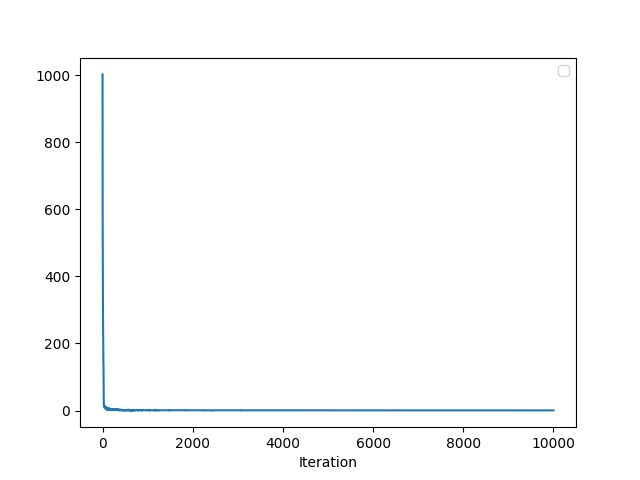
\includegraphics[width=.7\textwidth]{pic/Figure_9.png}
    \end{figure}
    可以看出几乎不需要10000次迭代,模型就会收敛。在UML一书上,作者给出了以下结论:
    \begin{equation}
        \sum_{t=1}^T(\mathbb{E}[f(\mathbf{w}^{(t)})]-f(\mathbf{w}^\star))\leq\frac{\rho^2}{2\lambda}\sum_{t=1}^T\frac{1}{t}\leq\frac{\rho^2}{2\lambda}(1+\log(T)) \nonumber
    \end{equation}
    故如此计算的收敛速度是$O(\frac{\log T}{T})$的。这远小于原先的$O(\frac{1}{\sqrt T})$。
\end{solution}

\begin{solution}{3.4.4}
    在实现中,曾尝试了\textbf{高斯核、双曲正切核以及线性核}。不知是因为我实现有误的原因,还是超参数调整不当,前两者的效果都非常差,故最后选择了线性核。即:
    \begin{equation}
        k(x, y) = x^\top y \nonumber
    \end{equation}
    \\
    学习率设置为$0.01$,正则化系数$\lambda = 0$,训练$100000$轮,最终在验证集上的准确率约为$0.7$。
\end{solution}


\begin{solution}{3.4.5}
    选取不带核函数的线性SVM作为最终的结果。学习率为$0.01$,正则化系数为$0.005$。验证集上准确率:$0.86$,F1-Score: $0.83$,混淆矩阵为:
    $$
    \begin{bmatrix}
        607 & 69 \\
        158 & 549 \\
    \end{bmatrix}
    $$
\end{solution}


\end{document}